
\documentclass[10pt, a4paper]{article}

\usepackage[top=1in, bottom=1in, left=1in, right=1in]{geometry}
%\usepackage{setspace}
%\onehalfspacing
\usepackage{graphicx}
\usepackage{float}

\usepackage{subfig}
\usepackage{amsmath}

\usepackage{amssymb}
\usepackage{fancyhdr}
\usepackage{listings}
\usepackage{textcomp}
\usepackage{upquote}
\pagestyle{fancyplain}

\renewcommand{\arraystretch}{1.5}

\begin{document}
\lhead{Jay Mundrawala}
\rhead{ECE 481 - Homework 1}

\section{Written}
\begin{enumerate}
  \item[\textbf{1a. }]
    \begin{equation} \label{eq:womix}
      \alpha_i(C) = \int C(\lambda) S_{i}(\lambda)\, d\lambda \\
    \end{equation}
    \begin{equation} \label{eq:wmix}
      \alpha_i(M) = \int \underbrace{\left[\sum_{k=1}^{2}\beta_{k}(C)P_{k}(\lambda) \right]}_{M(\lambda)}S_i(\lambda)\, d\lambda \\
    \end{equation}
    From \eqref{eq:womix}:
    \begin{eqnarray}
      \alpha_1(C) &=& \int^{6}_{5} \left( \frac{1}{2}\lambda -2 \right) \, d\lambda \\
      &=& \left[\frac{1}{4}\lambda^{2} - 2\lambda \right]^{6}_{5} + \left[\lambda \right]^{7}_{6} \\
      &=& \dfrac{3}{4} + 1 \\
      &=& \dfrac{7}{4}
    \end{eqnarray}
    \begin{eqnarray}
      \alpha_2(C) &=& \int^6_5 \left(\frac{1}{2}\right) \, d\lambda \\
      &=& \dfrac{1}{2}
    \end{eqnarray}
    If
    $P_1(\lambda) = \delta (\lambda-5)$
    and
    $P_2(\lambda) = \delta (\lambda-7)$
    then, from \eqref{eq:wmix}
    \begin{eqnarray}
      \alpha_1(M) &=& \int^6_4 \left[\beta_1\delta(\lambda-5) + \beta_2\delta(\lambda-7)\right]\left(\frac{1}{2}\lambda-2\right)\,
      d\lambda \\
      && + \int^8_6\left[\beta_1\delta(\lambda-5) + \beta_2\delta(\lambda-7)\right]\,d\lambda \nonumber \\
      &=& \left[\left(\dfrac{1}{2}\right)\beta_1 + \left(\dfrac{3}{2}\right)\beta_2\right] + \left[\beta_1 + \beta_2 \right] \\
      &=& \dfrac{3}{2}\beta_1 + \dfrac{5}{2}\beta_2 = \dfrac{7}{4}
    \end{eqnarray}
    \begin{eqnarray}
      \alpha_2(M) &=& \int^6_4\left[\beta_1\delta(\lambda-5) + \beta_2\delta(\lambda-7)\right]\left(\dfrac{1}{2}\right)\,d\lambda \\
      &=& \dfrac{1}{2}\beta_1 + \dfrac{1}{2}\beta_2 = \dfrac{1}{2}
    \end{eqnarray}
    Solving for $\beta_1$ and $\beta_2$
    \begin{eqnarray}
      \dfrac{3}{2}\beta_1 + \dfrac{5}{2}\beta_2 &=& \dfrac{7}{4} \\  
      \beta_1 + \beta_2 &=& 1 \\
      \beta_1 &=& \dfrac{3}{4} \\
      \beta_2 &=& \dfrac{1}{4}
    \end{eqnarray}
  \item[\textbf{1b. }]
    \begin{equation}
      \alpha_1(C) = \int^5_2\, d\lambda = 3
    \end{equation}
    \begin{equation}
      \alpha_2(C) = 4\int^3_1\, d\lambda = 8
    \end{equation}
    \begin{eqnarray}
      \alpha_1(M) &=& \int \left[\beta_1 P_1(\lambda) + \beta_2 P_2(\lambda)\right]S_1(\lambda)\, d\lambda \\
      &=& \int \beta_1 P_1(\lambda) S_1(\lambda)\, d\lambda + \int \beta_2 P_2(\lambda) S_1(\lambda)\, d\lambda \\
      &=& \beta_1 \int^6_5\, d\lambda + \beta_2 \int^4_2\, d\lambda \\
      &=& \beta_1 + 2\beta_2 = 3
    \end{eqnarray}
    \begin{eqnarray}
      \alpha_2(M) &=& \int \left[\beta_1 P_1(\lambda) + \beta_2 P_2(\lambda)\right]S_2(\lambda)\, d\lambda \\
      &=& \int \beta_1 P_1(\lambda) S_2(\lambda)\, d\lambda + \int \beta_2 P_2(\lambda) S_2(\lambda)\, d\lambda \\
      &=& 0 + 4\beta_2\int^3_2\, d\lambda = 4\beta_2 = 8
    \end{eqnarray}
    \begin{eqnarray}
      4\beta_2 &=& 8 \\
      \beta_2 &=& 2 \\
      \beta_1 &=& -1
    \end{eqnarray}

    This color is not achievable since there is a negative \beta, meaning it must be subtracted.

\end{enumerate}

\section{Computer Assignment}
The program for searching is listed in Listing \ref{code:search}. The code to separate an image into
its RGB channels is listed in Listing \ref{code:rgb}. Figure \ref{fig:q1} shows the results of q1.tif.
Figure \ref{fig:q2} shows the results of q2.tif. In both cases, the leftmost image is the query, followed
by the top result, and then the next best result.

\begin{figure}[h!]
  \centering
  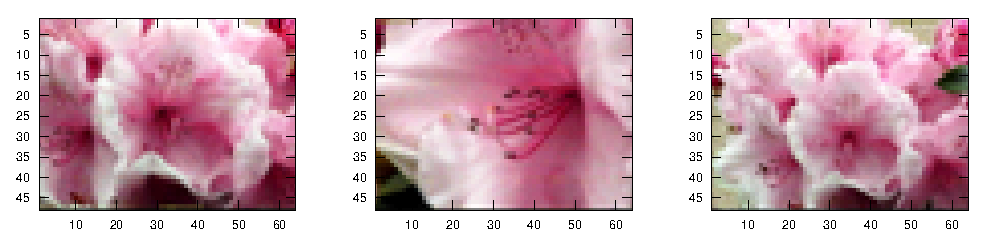
\includegraphics{../data/0.eps}
  \caption{Query q1.tif}
  \label{fig:q1}
\end{figure}

\begin{figure}[h!]
  \centering
  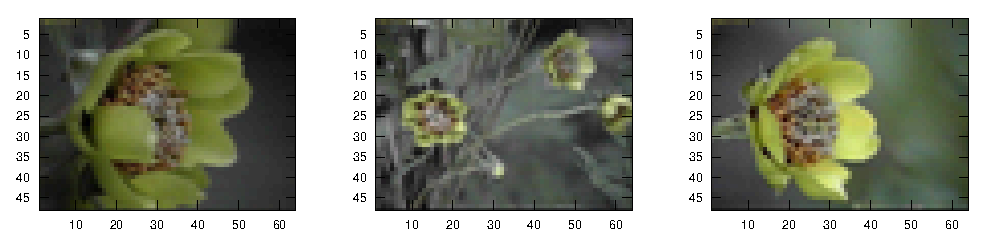
\includegraphics{../data/1.eps}
  \caption{Query q2.tif}
  \label{fig:q2}
\end{figure}

The colorplot3d program shows the 5 images in a 3D space. As expected, images 1 and 4 are close to each other
and 2 and 5 are close to each other. 1 and 4 seem like predominately green images, however the 3D space shows
that images 2 and 5 have a higher intensity of green. This can be explained by the amount of white in these 
images, which would also explain the high intensity of blue in those images. Image 1 and 3 are quite close to
each other even though they look nothing alike. That means that this search technique wont be very good if a
query was very similar to image 1, maybe with a little more red and blue in it. 

\begin{figure}[h!]
  \centering
  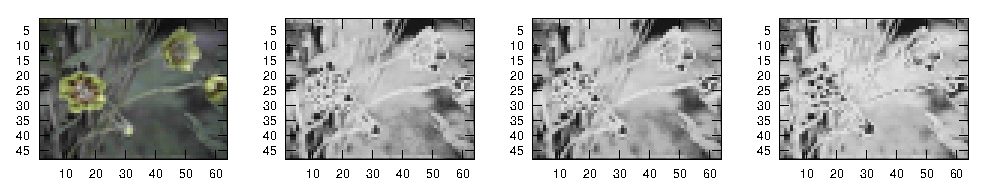
\includegraphics{../data/c0.eps}
  \caption{Image 1.tif along with its RGB channels}
  \label{fig:rgb}
\end{figure}

\pagebreak
\section{Code}
\lstset{ %
language=Octave,                % choose the language of the code
basicstyle=\footnotesize,
numbers=left,                   % where to put the line-numbers
stepnumber=1,                   % the step between two line-numbers. If it's 1 each line will be numbered
numbersep=10pt,                  % how far the line-numbers are from the code
showspaces=false,               % show spaces adding particular underscores
showstringspaces=false,         % underline spaces within strings
showtabs=false,                 % show tabs within strings adding particular underscores
frame=none,                    % adds a frame around the code
tabsize=2,                  % sets default tabsize to 2 spaces
captionpos=b,                   % sets the caption-position to bottom
breaklines=true,                % sets automatic line breaking
upquote=true,
breakatwhitespace=false        % sets if automatic breaks should only happen at whitespace
}

\lstset{caption=Search script,label=code:search}
\lstinputlisting{../src/search.m}

\lstset{caption=RGB Channel script,label=code:rgb}
\lstinputlisting{../src/rgb_chan.m}

\end{document}

